\documentclass[letterpaper]{article}

% AAAI-26 style. Place aaai2026.sty from the official AAAI author kit in
% this directory before compiling.
\usepackage[submission]{aaai2026}

\usepackage{times}
\usepackage{helvet}
\usepackage{courier}
\usepackage[hyphens]{url}
\usepackage{graphicx}
\urlstyle{rm}
\def\UrlFont{\rm}
\usepackage{natbib}
\usepackage{caption}
\usepackage{booktabs}
\usepackage{float}
\usepackage{amsmath}
\usepackage{amssymb}
\usepackage{listings}
\usepackage{xcolor}

\DeclareCaptionStyle{ruled}{labelfont=normalfont,labelsep=colon,strut=off}
\lstset{
  basicstyle={\footnotesize\ttfamily},
  breaklines=true,
  columns=fullflexible,
  keepspaces=true,
}

\pdfinfo{
/TemplateVersion (2026.1)
}

\setcounter{secnumdepth}{2}

\title{Consensus Is Not Completion: False Convergence in Multi-Agent Discovery Workflows}

\author{
    Anonymous Authors
}
\affiliations{
    Paper under anonymous review
}

\begin{document}

\maketitle

\begin{abstract}
Multi-agent language-model workflows often treat agreement, overlap, or a final
summary as evidence that a task is complete. This is unsafe in closed-world
discovery tasks, where the goal is to find all relevant items. We introduce
\emph{false convergence}: a workflow state in which agents report completion
and exhibit high agreement, yet the final answer omits true items. We identify
two mechanisms: \emph{aggregation loss}, where minority-discovered true items
are discarded during consensus or summarization, and \emph{common blind spots},
where agents agree because they miss the same region of the search space. We
argue that completion should be modeled as coverage-risk assessment under
correlated exploration rather than vote-counting. We implement a frozen
evidence-preserving staged audit controller that first audits singleton
evidence, then escalates to source-partitioned and boundary-focused review, and
otherwise abstains. Online experiments on Requests, held-out Click, and a new
held-out itsdangerous repository show that staged auditing improves recall over
singleton audit but trades precision and cost against simpler source review; on
itsdangerous it also produces one false certification. The evidence therefore
supports the mechanism and recall--cost value of preserving minority evidence,
but not a general safe-stopping claim. Broader benchmark validation, independent
oracle second review, and second-model replication remain open.
\end{abstract}

\begin{figure}[t]
\centering
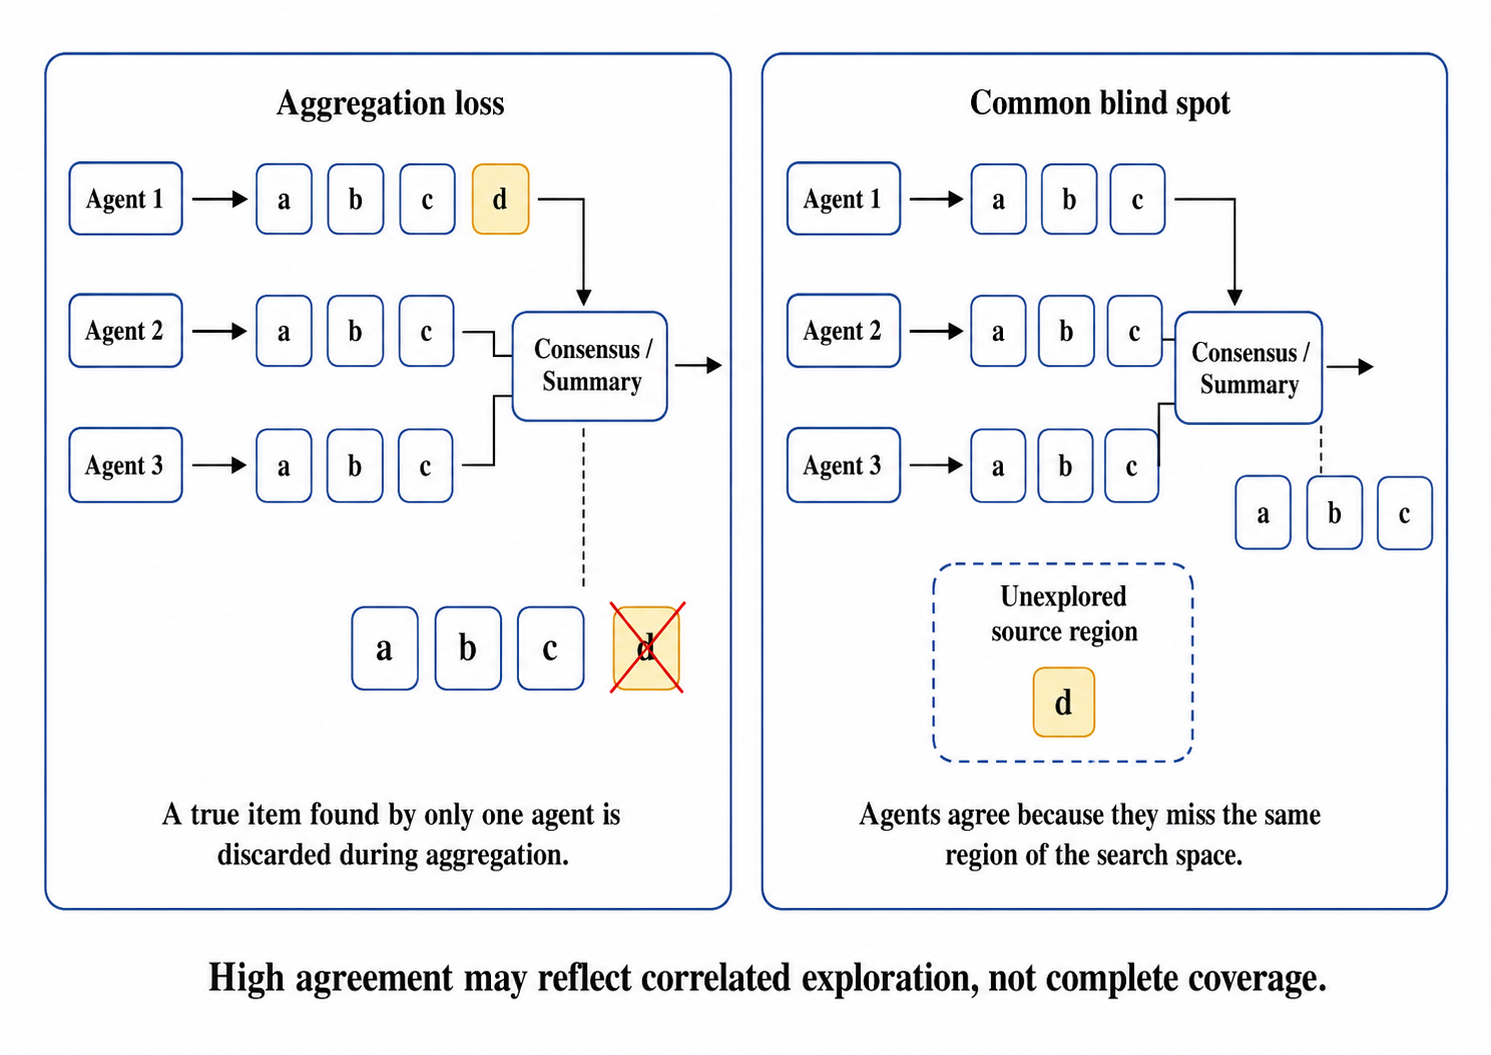
\includegraphics[width=0.95\columnwidth]{figures/false_convergence_mechanisms.png}
\caption{Two false-convergence mechanisms. Aggregation loss drops minority true
evidence during consensus or summarization; common blind spots arise when
agents agree because they miss the same source region.}
\label{fig:false-convergence}
\end{figure}

\begin{figure*}[t]
\centering
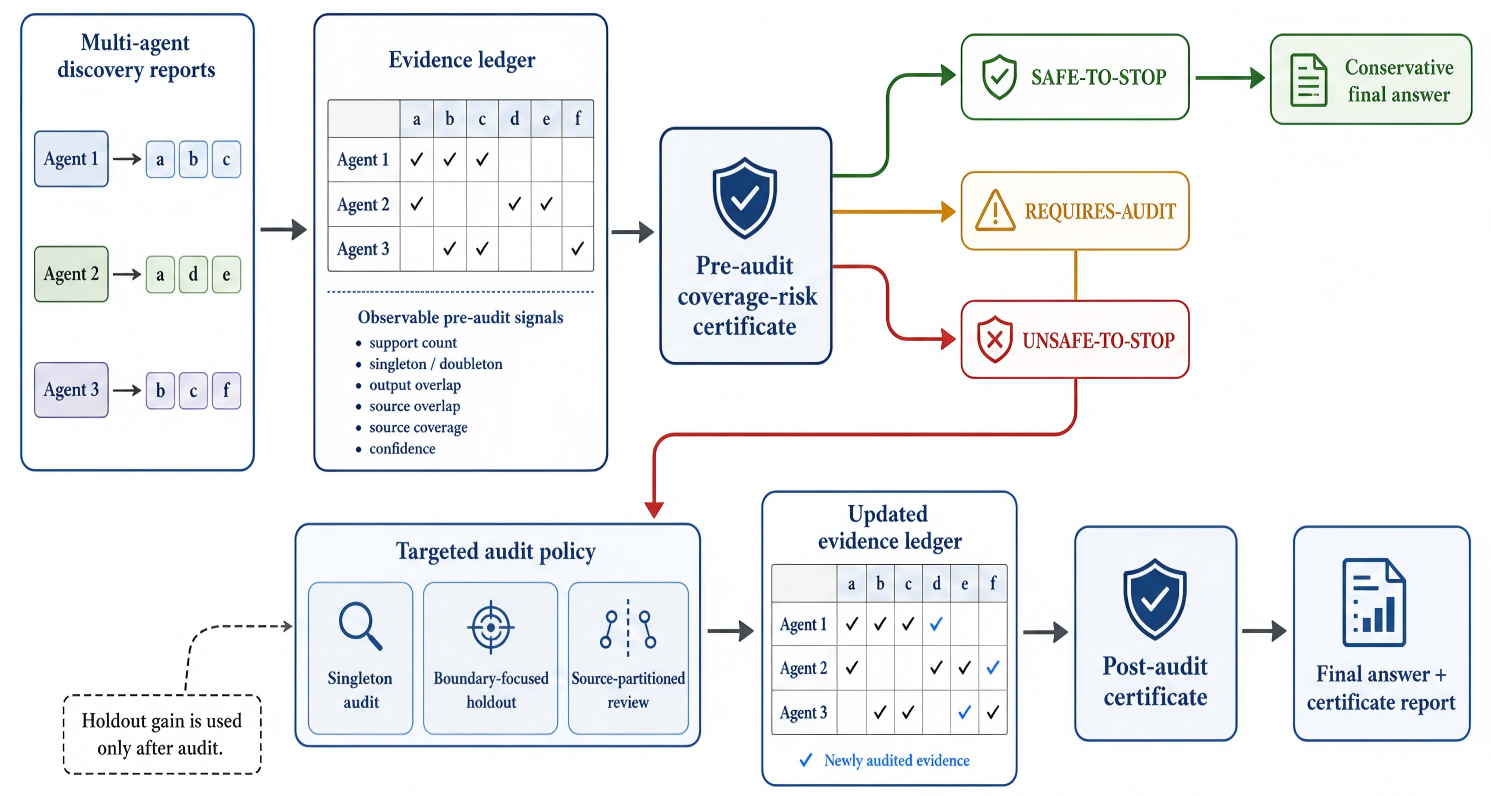
\includegraphics[width=0.90\textwidth]{figures/jiagou.png}
\caption{Decoupled completion workflow. The certificate decides whether the
workflow can stop; the audit policy decides how to recover missing evidence.
Holdout gain is not used as a pre-audit feature.}
\label{fig:workflow}
\end{figure*}

\section{Introduction}

Multi-agent language-model systems are increasingly used for tasks that require
search, decomposition, and synthesis. A common design pattern is simple:
multiple agents nominally inspect a task without shared intermediate answers,
their outputs are aggregated by
majority vote or a summarizer, and the system stops when agents agree or report
high confidence. This pattern is natural. Agreement is easy to measure, and
summaries provide a clean final answer.

However, agreement is not the same as completion. In closed-world discovery
tasks, such as finding every affected file location, every policy case, or every
relevant document in a bounded corpus, the central question is not only whether
the final answer is plausible. It is whether there remains missing mass outside
the discovered set. A group of agents can converge for the wrong reason: they
may share a search strategy, omit the same boundary cases, or discard minority
evidence during aggregation.

This paper studies this failure mode. We call it \emph{false convergence}: a
workflow state in which the system appears complete under its own completion
signals but is incomplete under a closed-world oracle. The failure is subtle
because the final output can have perfect precision and high self-reported
confidence. The error is not necessarily hallucination. It is often omission.

We make three contributions.

\begin{itemize}
    \item We define false convergence in closed-world agentic discovery and
    distinguish two mechanisms: aggregation loss and common blind spots.
    \item We propose an evidence-preserving staged audit controller that
    separates recovery from certification: singleton and source evidence can be
    audited without declaring the workflow complete.
    \item We provide online recall--cost evidence on Requests, held-out Click,
    and held-out itsdangerous, together with bootstrap paired comparisons and
    negative evidence about safe stopping.
\end{itemize}

Our results do not imply that union aggregation is always better than consensus.
Instead, they show that singleton evidence has two faces. Sometimes it is
missing mass; sometimes it is noise. A reliable completion controller should
model this distinction rather than silently deleting minority evidence or
blindly accepting all unique items.

\section{Related Work}

\subsection{Multi-Agent Consensus, Aggregation, and Calibration}

Self-consistency selects a consistent answer from multiple samples
\citep{wang2022selfconsistency}; debate, collaboration, and role-specialized
agent frameworks improve reasoning or task performance
\citep{du2023debate,chan2023chateval,wu2023autogen,chen2023agentverse,
hong2023metagpt,li2023camel,zhang2024proagent}. Recent work also studies
majority-failure auditing, selection bottlenecks, trace-level synthesis, and
calibration under communication-induced correlation
\citep{yang2026agentauditor,maryanskyy2026agentsdisagree,
fadnavis2026beyondconsensus,huang2026cagecal}. Tool-using and
planning agents extend LLMs through environment interaction
\citep{yao2023react,schick2023toolformer,qin2023toolllm,yao2023tot,
wang2023voyager}. Benchmarks such as
AgentBench, WebArena, GAIA, and SWE-bench stress interactive or software tasks
\citep{liu2023agentbench,zhou2023webarena,mialon2023gaia,jimenez2023swebench}.
Our focus is different: aggregation is judged by closed-world recall and
calibrated stopping risk, not by the quality of one selected answer.

\subsection{Wide Research and Completeness Evaluation}

Self-Refine, Reflexion, CRITIC, Chain-of-Verification, and related factuality
checks repair or verify outputs
\citep{madaan2023selfrefine,shinn2023reflexion,gou2023critic,dhuliawala2023cov,
lin2021truthfulqa,manakul2023selfcheckgpt,li2023halueval}. Retrieval-augmented
generation and dense retrieval reduce hallucination but still face noise,
negative rejection, integration, and long-context failures
\citep{lewis2020rag,guu2020realm,karpukhin2020dpr,nakano2021webgpt,
chen2024rgb,li2024unigen,liu2023lost,asai2023selfrag,
gao2023ragsurvey}. Closed-world discovery is also related to high-recall
retrieval, fact verification, and technology-assisted review, where stopping is
a coverage-estimation problem
\citep{thorne2018fever,yang2018hotpotqa,grossman2015trec,
cormack2021tarstopping}. Our certificate adopts this stopping perspective for
correlated LLM-agent exploration.
Recent broad or deep research benchmarks explicitly evaluate exhaustive
information seeking and stopping uncertainty
\citep{wong2025widesearch,gupta2026deepsearchqa,rafiee2026trqa,
huang2026wideseek,kim2026seekergym}.

\subsection{Coverage Estimation and Stopping}

Our certificate uses observable missing-mass signals rather than oracle labels at
decision time. Singleton counts and unseen-mass estimates are conceptually
related to Good-Turing, Chao-style, capture-recapture, and ecological diversity
estimators \citep{good1953population,chao1984nonparametric,
mcAllester2000goodturing,chao2014rarefaction,bron2024chao}. Recent LLM and
multi-agent uncertainty methods
estimate answer risk from probabilities, samples, or semantic variation
\citep{kuhn2023semanticentropy,kadavath2022language,chen2026matu,
cole2023selectively}. We study a complementary question: whether a multi-agent
workflow has covered a bounded item set well enough to stop.

\section{Problem Formulation}

\subsection{Closed-World Discovery Tasks}

We consider tasks with a bounded source collection $D$ and a finite oracle set
$Y^\star$ of target items. A run returns a set $\hat{Y}$. We evaluate:

\begin{align}
\text{Recall}(\hat{Y}) &= \frac{|\hat{Y} \cap Y^\star|}{|Y^\star|}, \\
\text{Precision}(\hat{Y}) &= \frac{|\hat{Y} \cap Y^\star|}{|\hat{Y}|}.
\end{align}

Examples include code dependency audits, policy-case discovery, high-recall
document review, and bounded repository analysis. Unlike open-ended question
answering, a plausible final answer is insufficient: the system must decide
whether it has found the complete set.

\subsection{Multi-Agent Completion Signals}

A typical workflow runs $k$ agents $A_1, \ldots, A_k$, each producing an item set
$Y_i$, a completion flag $c_i$, and a confidence score $q_i$. Aggregation then
produces a final set $Y_{\text{agg}}$. Common aggregation rules include:

\begin{itemize}
    \item \textbf{Majority consensus}: keep items reported by at least two
    agents.
    \item \textbf{Standard summarization}: ask a summarizer to produce a clean
    final answer from the agent reports.
    \item \textbf{Raw union}: keep every unique item reported by any agent.
    \item \textbf{Union-preserving summarization}: instruct a summarizer to
    preserve all unique reported items unless malformed or contradicted.
\end{itemize}

Systems often treat high pairwise overlap, high mean confidence, and affirmative
self-reported completion as stopping evidence. We argue that these are not
completion certificates.

\subsection{False Convergence}

Let $S$ be a multi-agent workflow state with $k$ agents, an aggregation rule
$g$, and a target recall threshold $\theta$. We say $S$ exhibits false
convergence under $g$ when:

\begin{enumerate}
    \item agents self-report completion with high confidence;
    \item agent outputs exhibit high overlap;
    \item the aggregated answer $g(Y_1,\ldots,Y_k)$ has recall below $\theta$.
\end{enumerate}

Our fixed evaluation protocol uses $\theta=0.95$, confidence threshold $0.80$, and
overlap threshold $\tau=0.70$. Holdout recovery is a diagnostic and audit
mechanism, not part of the definition. We also report near-positive and
mechanism-positive cases when the missing items are few but diagnostically
important.

\subsection{Aggregation Loss}

Aggregation loss occurs when a true item appears in at least one agent report
but is removed by consensus-style aggregation or standard summarization. This is
not a search failure: the evidence exists in the reports. The failure happens at
the final synthesis step.

Formally, an oracle item $y \in Y^\star$ is an aggregation-loss item if:
\begin{equation}
y \in \bigcup_i Y_i \quad \text{and} \quad y \notin Y_{\text{agg}}.
\end{equation}
When $y$ appears in only one agent report, it is a singleton true positive.

\subsection{Common Blind Spots}

Common blind spots occur when multiple agents agree because they share a search
failure. In this case, the missing item is absent even from the raw union:
\begin{equation}
y \in Y^\star \quad \text{and} \quad y \notin \bigcup_i Y_i.
\end{equation}
Raw union and union-preserving summarization cannot recover such items because
there is no reported evidence to preserve. The mitigation must change the search
or auditing process, for example through boundary-focused holdout review.

\subsection{Singletons as Missing Mass or Noise}

Singletons are ambiguous. A singleton may be a hard-to-find true positive, or it
may be a false positive. Consensus implicitly treats singletons as noise. Raw
union implicitly treats them as valid evidence. Both assumptions are unsafe. The
right action is often to preserve singleton evidence for audit.

\section{Evidence-Preserving Staged Audit Controller}

We propose a staged audit controller for deciding whether a multi-agent
discovery workflow can safely stop or should preserve evidence for further
review. A lightweight completion certificate is the controller's risk-triage
module. It is not an oracle: it does not use ground truth and does not decide
final item labels. Instead, it maps observable workflow signals to a stopping
or escalation judgment.

\subsection{Controller Inputs and Decisions}

The controller takes only pre-audit observable logs: agent item sets, support
counts, confidence, source-family metadata, and source coverage. It never uses
oracle labels, task identifiers, repository identifiers, post-audit gain, or
holdout outcomes as decision features. Its labels are
\textsc{safe-to-stop}, \textsc{requires-audit}, and \textsc{unsafe-to-stop};
false-certification rate and safe coverage are therefore reported separately.
The older v1/v2 risk formulas and leakage audits are in the supplementary
appendix rather than promoted as the main method.

\subsection{Evidence-Preserving Audit Policy}

When the certificate returns \textsc{unsafe-to-stop} or
\textsc{requires-audit}, the workflow needs an audit policy. We use an
evidence-preserving policy that separates finalization from evidence retention:
consensus items form a conservative answer, singleton evidence is retained for
review, and high-agreement boundary-risk states trigger holdout or source-focused
audit. This policy is the audit response to a risky certificate state, not the
certificate itself.

The audit policy handles the two failure mechanisms differently. For aggregation
loss, it preserves and audits singleton or minority evidence instead of deleting
it during summarization. For common blind spots, where no current agent reported
the missing item, it triggers boundary-focused holdout or source-focused review.
In our experiments, singletons are not automatically accepted; they are retained
and audited. High agreement is not automatically trusted; it can trigger a
common-blind-spot check. The full procedural listing is in the supplementary
appendix.

The frozen staged controller used after the Requests development experiment
therefore applies a simple order: conservative consensus, singleton verifier,
source-partitioned review when singleton mass, union gap, or source-family gaps
remain, and abstention if escalation was needed. This makes recovery and
certification separate: the controller may recover true positives while still
refusing to certify completion.

\begin{table}[t]
\centering
\footnotesize
\begin{minipage}{0.96\columnwidth}
\textbf{Algorithm 1: Evidence-Preserving Staged Audit Controller}

\begin{enumerate}
    \item Input blind reports $Y_1,\ldots,Y_k$ and pre-audit source metadata.
    \item Set $F=\{y:n(y)\ge2\}$ and singleton queue $Q=\{y:n(y)=1\}$.
    \item If $Q$ is non-empty, run the frozen singleton verifier and add
    verified items to $F$.
    \item If singleton ratio, consensus--union gap, or source-family coverage
    gaps remain, run source-partitioned review and add verified items to $F$.
    \item If the task declares boundary-sensitive families and unresolved
    evidence remains, run boundary-focused holdout.
    \item Return \textsc{safe-to-stop} only when no trigger remains, required
    families are represented, confidence is at least .75, and all discovery
    agents reported completion.
    \item Otherwise return the recovered set with \textsc{requires-audit} or
    \textsc{unsafe-to-stop}; do not certify completion.
\end{enumerate}
\end{minipage}
\caption{Frozen staged controller used for held-out online validation. Oracle
labels are never used by the controller; they are used only after logging for
offline scoring.}
\label{alg:staged-controller}
\end{table}

\section{Experimental Setup}

\subsection{Research Questions}

We ask:

\begin{itemize}
    \item \textbf{RQ1}: Can consensus-style aggregation produce false completion
    signals in closed-world discovery tasks?
    \item \textbf{RQ2}: Are failures caused by aggregation loss, common blind
    spots, or both?
    \item \textbf{RQ3}: Does raw union solve the problem, or does it introduce a
    precision cost?
    \item \textbf{RQ4}: Can a coverage-risk certificate identify unsafe
    stopping states, and when can an audit policy recover missing items?
\end{itemize}

\subsection{Tasks}

We use five bounded discovery task families: two synthetic families designed to
isolate mechanisms, two real-repository audits used during method development
and held-out validation, and one additional public repository introduced only
after the staged controller was frozen.

\textbf{T1: Code dependency audit.} Agents inspect a synthetic AcmePay migration
repository and must find every code or configuration location that resolves to
AcmePay v1 through direct calls, routing configuration, registry indirection,
fallback queues, or replay scripts. The hard oracle has 35 items.

\textbf{T2: Policy document search.} Agents inspect naturalistic incident notes,
changelogs, appendices, and policy memos. They must find all cases whose state,
flow, and service-resolution chain imply AcmePay v1 handling. The oracle has 30
items. Boundary cases require following service catalog and adapter registry
resolution rather than relying on surface service names.

\textbf{T3: Real-repository Click deprecation audit.} Agents inspect a fixed
snapshot of the public Click repository and must find line-level locations that
belong to a deprecated API surface audit. The oracle has 149 items spanning
implementation, warning emission, help-message formatting, parameter behavior,
tests, documentation, and bounded changelog entries. Unlike T1/T2, T3 uses a
real repository and is used as a stronger validation of aggregation behavior
rather than as a strict false-convergence construction.

\textbf{T4: Real-repository Requests TLS audit.} We additionally instantiate a
second real-repository task family from a fixed snapshot of the public Requests
repository. The task asks agents to find line-level items related to TLS
certificate verification, CA bundle resolution, client certificates, SSL error
handling, tests, test infrastructure, and user documentation. The oracle has
304 items. T4 is used to test whether the real-repository result depends on
Click or deprecation-surface search.

\textbf{T5: Real-repository itsdangerous timed-signing audit.} For external
validation, we add a previously unused public repository, itsdangerous, fixed at
commit \texttt{672971d}. The task asks agents to find bounded line-level items
related to timestamped signing, max-age expiration, \texttt{SignatureExpired},
\texttt{TimestampSigner}, \texttt{TimedSerializer}, tests, documentation,
exports, and changelog entries. The initial oracle has 160 items and still
requires independent second review.

\subsection{Runs and Aggregation Policies}

Each seed contains three G3 agents. Where available, we also run an independent
G6 holdout scout. To test whether the certificate simply always refuses to stop,
we construct mixed evaluation states from saved logs: each single agent, each
two-agent union, the three-agent pre-audit union, and the post-holdout state
when available. This yields complete, near-complete, and incomplete states
without generating new oracle-dependent agent outputs. We compare:

\begin{itemize}
    \item majority consensus;
    \item blind standard summarization;
    \item raw union;
    \item blind union-preserving summarization;
    \item holdout scout;
    \item self-reported completion, confidence-only, overlap-only, no-new-item,
    Chao-only, always-unsafe, always-holdout, and the proposed certificate.
\end{itemize}

The standard and union-preserving summarizers are blind to oracle and scoring
files. The pre-audit certificate uses only exploration outputs and metadata;
holdout gain is used only after audit. Oracle is used only for offline metrics.

\subsection{Closed-Loop Evaluation and Data Volume}

The experiment is designed as a closed loop rather than a collection of isolated
case studies. Each task has a bounded source collection and oracle. Each run
produces agent item sets and metadata. Aggregation policies produce candidate
answers. The pre-audit certificate decides whether the state is safe, unsafe, or
requires audit without access to oracle labels or holdout gain. Audit policies
then update the evidence ledger, and final recall, precision,
false-certification rate, audit recovery, and cost metrics are computed offline.
This loop lets us evaluate both failure diagnosis and the downstream control
decision.

The online blind LLM evidence covers three-agent seeds on two synthetic task
families and three real-repository audits. Requests uses five seeds and four
discovery configurations for audit-policy development. After that stage, the
controller is frozen and evaluated on held-out Click and external itsdangerous
online grids without retuning. Full data-volume tables, v1/v2 diagnostics, and
log paths are in the supplementary appendix.

\section{Results}

\begin{figure*}[t]
\centering
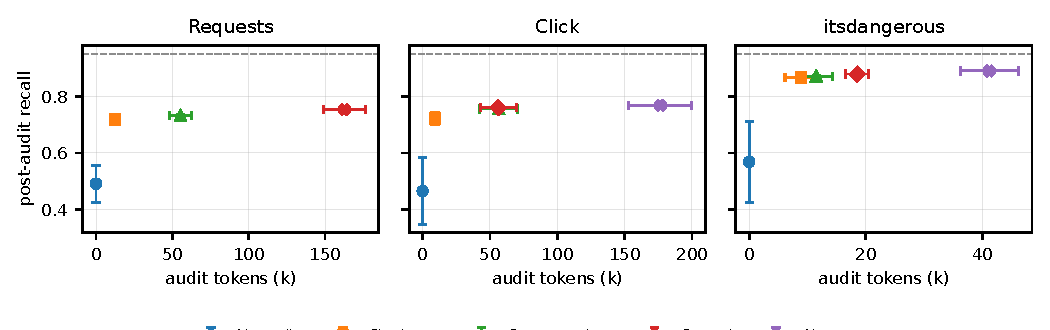
\includegraphics[width=0.98\textwidth]{figures/multi_repo_recall_cost.pdf}
\caption{Online recall--cost tradeoffs on Requests, held-out Click, and
external itsdangerous. The dashed line marks the 0.95 recall threshold used for
safe-state analysis. Requests is a development audit-policy suite and has no
frozen staged-controller arm.}
\label{fig:online-audit-pareto}
\end{figure*}

\subsection{Mechanism Evidence}

The six mechanism slices show the two failure modes. T1 seed01 and
T2 seed01 show aggregation loss: true items were present in minority reports but
dropped by consensus and standard summaries. T2 seed02 and seed03 show common
blind spots: all three G3 agents agreed on the same incomplete 28-item set, and
raw union could not recover the missing cases. T1 seed02 and seed03 are
precision-cost controls: consensus is complete, while raw union preserves false
positive singletons.

\subsection{Aggregation Policy Comparison}

Consensus and standard summarization can produce high-precision false stops.
Raw union and union-preserving summarization recover aggregation-loss cases, but
incur precision cost in T1 seed02/03 and cannot recover T2 common blind spots.
The evidence-preserving audit policy recovers missing items when holdout
evidence is available and marks singleton-noise controls as requiring audit.
Full per-slice tables are in the supplementary appendix.

\subsection{Real-Repository Summarizer False Stops}

T3 evaluates whether the aggregation-stage failure appears in a real repository
task rather than only in constructed mechanism slices. We give the same G3
aggregation packet to two blind LLM summarizers. The \emph{standard} summarizer
is instructed to produce a concise, high-precision final answer from the three
agent reports. The \emph{union-preserving} summarizer is instructed to preserve
all unique reported items unless malformed or contradicted.

Table~\ref{tab:t3-summarizers} shows a stable pattern across three blind seeds.
The standard summarizer reports completion with confidence between 0.93 and
0.96, but its recall is only 0.685--0.745. Its precision is nearly perfect, so
the failure is not hallucination; it is omission. The union-preserving
summarizer removes the false stop in all three seeds, reaching 0.993--1.000
recall, but precision falls to 0.639--0.744. This supports two claims. First,
much of the missing evidence was already present in the agent reports and was
discarded during aggregation. Second, naive union preservation is diagnostic but
not a complete solution because it preserves noise along with missing true
items.

\begin{table*}[t]
\centering
\small
\begin{tabular}{llrrrrrrr}
\toprule
Seed & Policy & Conf. & Found & TP & FP & Recall & Precision & False Stop \\
\midrule
01 & standard summarizer & 0.930 & 105 & 104 & 1 & 0.698 & 0.990 & yes \\
01 & union-preserving summarizer & 0.910 & 199 & 148 & 51 & 0.993 & 0.744 & no \\
02 & standard summarizer & 0.960 & 111 & 111 & 0 & 0.745 & 1.000 & yes \\
02 & union-preserving summarizer & 0.950 & 233 & 149 & 84 & 1.000 & 0.639 & no \\
03 & standard summarizer & 0.930 & 102 & 102 & 0 & 0.685 & 1.000 & yes \\
03 & union-preserving summarizer & 0.840 & 232 & 149 & 83 & 1.000 & 0.642 & no \\
\midrule
Mean & standard summarizer & -- & -- & -- & -- & 0.709 & 0.997 & 3/3 \\
Mean & union-preserving summarizer & -- & -- & -- & -- & 0.998 & 0.675 & 0/3 \\
\bottomrule
\end{tabular}
\caption{T3 real-repository summarizer comparison. The oracle contains 149
line-level Click deprecation-audit items. Standard summarization is
high-precision but repeatedly false-stops; union-preserving summarization
recovers recall but incurs a substantial precision cost.}
\label{tab:t3-summarizers}
\end{table*}

\subsection{Second Real-Repository Task Family}

T4 evaluates a different real repository and audit surface: TLS and certificate
handling in Requests. Unlike T3, this task is larger and noisier. Table
~\ref{tab:t4-realrepo} shows that the failure shifts from mostly aggregation
loss to mixed search-coverage and aggregation risk. Majority consensus is
incomplete in all three seeds, with recall between 0.678 and 0.701. Raw union
improves recall to 0.829--0.859, showing that some omitted evidence is present
in minority reports, but raw union remains below the 0.95 completion threshold
in every seed. Thus T4 contains candidate-pool missing mass that union
aggregation cannot recover.

The standard summarizer also false-stops in all three seeds, with recall
0.368--0.648 despite self-reported completion. The completion certificate marks
all three seeds \textsc{unsafe-to-stop}. This supports the broader claim that a
completion controller must estimate coverage risk, not merely summarize or vote
over the current reports. T4 should not be read as a direct copy of the T3
mechanism; instead, it is a harder boundary case showing that real-repository
discovery can combine aggregation loss, noisy singleton evidence, and
insufficient search coverage.

\begin{table*}[t]
\centering
\small
\begin{tabular}{lrrrrrr}
\toprule
Seed & Cons. Rec. & Std. Rec. & Union Rec. & Union Prec. & Holdout Rec. & Cert. \\
\midrule
01 & 0.701 & 0.368 & 0.859 & 0.661 & 0.750 & unsafe \\
02 & 0.678 & 0.622 & 0.845 & 0.668 & 0.688 & unsafe \\
03 & 0.678 & 0.648 & 0.829 & 0.676 & 0.763 & unsafe \\
\midrule
Mean & 0.685 & 0.546 & 0.844 & 0.668 & 0.734 & 3/3 unsafe \\
\bottomrule
\end{tabular}
\caption{T4 Requests TLS/certificate audit on a second real repository. Raw
union improves over consensus but remains incomplete, indicating missing mass
outside the G3 candidate pool. Standard summarization false-stops in all three
seeds.}
\label{tab:t4-realrepo}
\end{table*}

\subsection{Decoupled Certificate and Stopping Baselines}

We then evaluate the decoupled v1 certificate on 96 saved states constructed
from existing runs: 86 pre-audit states and 10 post-audit states. Oracle labels
are used only for evaluation; a state is safe when recall is at least 0.95. The
suite contains 44 safe and 52 unsafe states. Table~\ref{tab:v1-certificate}
shows that simple stopping signals false-certify many incomplete states:
self-reported completion and confidence-only stopping each false-certify 35
states, Chao-only false-certifies 13, and overlap-only false-certifies 10. The
proposed certificate certifies one post-audit state and makes no false
certifications, but its safe coverage is only 0.023. Thus the current rule is a
conservative risk detector, not a solved stopping policy. Its continuous risk
score has AUROC 0.515 and AUPRC 0.589 for unsafe-state detection, indicating
that stronger correlation and coverage features are still needed.

\begin{table}[H]
\centering
\small
\begin{tabular}{lrrrr}
\toprule
Rule & Stop & False & FCR & Safe Cov. \\
\midrule
Self-report & 70 & 35 & .500 & .795 \\
Confidence & 70 & 35 & .500 & .795 \\
Overlap & 15 & 10 & .667 & .114 \\
No-new-item & 22 & 10 & .455 & .273 \\
Chao-only & 26 & 13 & .500 & .295 \\
Raw union & 86 & 49 & .570 & .841 \\
Always unsafe & 0 & 0 & .000 & .000 \\
Always holdout & 10 & 3 & .300 & .159 \\
Ours v1 & 1 & 0 & .000 & .023 \\
\bottomrule
\end{tabular}
\caption{Stopping evaluation on 96 mixed saved states. FCR is false
certification rate among stopped/certified states. The proposed certificate is
safe but too conservative in this version.}
\label{tab:v1-certificate}
\end{table}

\subsection{Transferability Audit of v2}

We freeze v1 and the v2 offline diagnostic before further inspection. A leakage
audit finds no direct use of oracle labels, holdout gain, task id, repository id,
or post-audit cost columns in the declared v2 feature set. However, a
metadata-only shortcut probe has high in-distribution AUROC, and
leave-one-repository-out validation fails to certify any held-out repository
under the same calibration rule: AUROC is .591 for Click, .546 for policy docs,
and .695 for Requests, with zero certified held-out states. Thus v2 remains an
offline diagnostic rather than the main method; the full leakage and
generalization table is in the supplementary appendix.

\subsection{Online Audit-Controller Evaluation}

We run the Requests TLS online audit-controller suite with a fixed model,
repository commit, prompt family, budget, and seeds 04--08. Each seed has four
blind discovery configurations: homogeneous, prompt-diverse, source-partitioned,
and independent-context. We then evaluate seven audit policies using only
pre-audit discovery logs to build audit queues. Online singleton and random
verifiers review candidate line snippets; boundary-focused holdout agents run a
separate blind search. Oracle labels are used only after audit evidence is
written.

\begin{table}[H]
\centering
\scriptsize
\resizebox{\columnwidth}{!}{
\begin{tabular}{lrrrrrr}
\toprule
Policy & Pre R & Post R & Prec. & Rec. TP & Intro. FP & Tok. \\
\midrule
No audit & .491 & .491 & .829 & 0.0 & 0.0 & 0k \\
Random holdout & .491 & .554 & .755 & 18.9 & 11.9 & 17k \\
Singleton audit & .491 & .719 & .725 & 69.1 & 38.7 & 12k \\
Boundary holdout & .491 & .694 & .755 & 61.7 & 24.6 & 71k \\
Source-partitioned review & .491 & .733 & .730 & 73.3 & 38.5 & 55k \\
Risk-triggered audit & .491 & .733 & .713 & 73.3 & 45.5 & 83k \\
Always holdout & .491 & .753 & .706 & 79.5 & 51.1 & 163k \\
\bottomrule
\end{tabular}}
\caption{Online Requests TLS audit-policy results averaged over 20
seed/configuration states. Pre R is the conservative consensus answer; union
items are retained as an evidence queue and enter the final answer only after
audit. Tokens are additional audit tokens, not discovery tokens.}
\label{tab:online-audit}
\end{table}

Table~\ref{tab:online-audit} and Figure~\ref{fig:online-audit-pareto} show that
auditing materially improves recall, but does not solve completion. Singleton
audit is the cheapest strong recovery mechanism because many missed true items
are already present as minority evidence. Source-partitioned review and
risk-triggered audit reach similar mean recall, while always-holdout buys the
highest recall at much higher cost. All policies remain below the 0.95
completion threshold, so the controller should continue to report
\textsc{unsafe-to-stop} rather than certify completion.

We then freeze the staged controller and evaluate it on held-out Click online
runs with three new seeds and three discovery configurations. The staged
controller reaches mean recall .761 versus .768 for always-holdout, while using
56k rather than 177k additional audit tokens. However, it abstains on every
held-out state, yielding zero false certifications but also zero safe coverage.
Thus the held-out result supports recall--cost recovery and reliable abstention,
not automatic safe stopping.

Finally, we add a previously unused public repository, itsdangerous, after the
controller is frozen. On this external task, staged control reaches mean recall
.879, compared with .867 for singleton audit, .871 for source-partitioned
review, and .890 for always-holdout. This is a useful recovery gain over
singleton audit, but it is not a clean dominance result: source-partitioned
review has higher precision and F1 at lower cost, and the staged controller
incorrectly certifies one unsafe state. A safe-state sweep with three additional
boundary-focused agents on seed04 spends 39.6k audit tokens, recovers only one
additional true positive, introduces three false positives, and raises recall
from .894 to only .900; no online safe state is reached.

Seed-clustered bootstrap paired comparisons over Click and itsdangerous show
that staged control improves recall over singleton audit by .025
([.012,.039]) but reduces precision by .042 and F1 by .013. Against
source-partitioned review, the recall gain is small, .007 ([.005,.009]), again
with lower precision and F1. Against always-holdout, staged control saves about
71k audit tokens on average but has lower recall by .009. We therefore treat
the staged controller as the current evidence-preserving method, not as a
solved safe-completion policy.

\section{Discussion and Limitations}

Consensus can be too conservative when a minority report contains real evidence
and too confident when agents share a blind spot. Raw union exposes aggregation
loss, but preserves singleton false positives and cannot recover unreported
items. Completion therefore needs coverage-risk control, not only vote counting.

The evidence supports mechanism-level claims and recall--cost recovery, not a
general proof of safe completion. v2 fails held-out repository/task-family
validation and remains supplementary. The frozen staged controller improves
recall over singleton audit, but external itsdangerous validation produces one
false certification and zero safe coverage; an extra boundary sweep still does
not reach .95 recall. Click, Requests, and itsdangerous also require independent
oracle second review, and second-model plus SeekerGym/TRQA/WideSearch benchmark
runs remain TODO until manifests, logs, and scores exist.

\section{Conclusion}

Consensus is not completion. We identified aggregation loss and common blind
spots as distinct reasons why high agreement can still omit true items. The
current online audit-controller results show that targeted audit can recover
missing true positives with measured cost, and that a frozen staged controller
can organize singleton and source review without using oracle labels. They also
show that recovery is not yet completion: external validation still produces no
safe coverage and one false certification. The next methodological step is a
stricter certification rule validated on independently reviewed external
oracles and public exhaustive-search benchmarks.

\bibliography{references}
\end{document}
